% This is "bach-ref-2009.tex" Updated january 29th 2010.
% This file should be compiled with "sig-alternate-fixed.cls" January 2010.
% It is based on the ACM style "sig-alternate.cls"
% -------------------------------------------------------------------------
% This example file demonstrates the use of the 'sig-alternate-fixed.cls'
% V2.5 LaTeX2e document class file. It is for those submitting
% articles to the Twente Student Conference on IT. Both this file as the
% document class file are based upon ACM documents.
%
% ----------------------------------------------------------------------------------------------------------------
% This .tex file (and associated .cls) produces:
%       1) The Permission Statement
%       2) The Conference (location) Info information
%       3) The Copyright Line TSConIT
%       4) NO page numbers
%       5) NO headers and/or footers
%
%
% Using 'sig-alternate.cls' you have control, however, from within
% the source .tex file, over both the CopyrightYear
% (defaulted to 200X) and the ACM Copyright Data
% (defaulted to X-XXXXX-XX-X/XX/XX).
% e.g.
% \CopyrightYear{2007} will cause 2007 to appear in the copyright line.
% \crdata{0-12345-67-8/90/12} will cause 0-12345-67-8/90/12 to appear in the copyright line.
%
% ---------------------------------------------------------------------------------------------------------------
% This .tex source is an example which *does* use
% the .bib file (from which the .bbl file % is produced).
% REMEMBER HOWEVER: After having produced the .bbl file,
% and prior to final submission, you *NEED* to 'insert'
% your .bbl file into your source .tex file so as to provide
% ONE 'self-contained' source file.
%

% refers to the cls file being used
\documentclass{sig-alternate-br}

\begin{document}
%
% --- Author Metadata here --- DO NOT REMOVE OR CHANGE
\conferenceinfo{23$^{th}$ Twente Student Conference on IT}{June 22$^{st}$, 2015, Enschede, The Netherlands.}
\CopyrightYear{2015} % Allows default copyright year (200X) to be over-ridden - IF NEED BE.
%\crdata{0-12345-67-8/90/01}  % Allows default copyright data (0-89791-88-6/97/05) to be over-ridden - IF NEED BE.
% --- End of Author Metadata ---

\title{Face spoofing detection on mobile phones in a user-friendly manner.}
% In Bachelor Referaat at University of Twente the use of a subtitle is discouraged.
% \subtitle{[Instructions]}

%
% You need the command \numberofauthors to handle the 'placement
% and alignment' of the authors beneath the title.
%
% For aesthetic reasons, we recommend 'three authors at a time'
% i.e. three 'name/affiliation blocks' be placed beneath the title.
%
% NOTE: You are NOT restricted in how many 'rows' of
% "name/affiliations" may appear. We just ask that you restrict
% the number of 'columns' to three.
%
% Because of the available 'opening page real-estate'
% we ask you to refrain from putting more than six authors
% (two rows with three columns) beneath the article title.
% More than six makes the first-page appear very cluttered indeed.
%
% Use the \alignauthor commands to handle the names
% and affiliations for an 'aesthetic maximum' of six authors.
% Add names, affiliations, addresses for
% the seventh etc. author(s) as the argument for the
% \additionalauthors command.
% These 'additional authors' will be output/set for you
% without further effort on your part as the last section in
% the body of your article BEFORE References or any Appendices.

\numberofauthors{1} %  in this sample file, there are a *total*
% of EIGHT authors. SIX appear on the 'first-page' (for formatting
% reasons) and the remaining two appear in the \additionalauthors section.
%
\author{
% You can go ahead and credit any number of authors here,
% e.g. one 'row of three' or two rows (consisting of one row of three
% and a second row of one, two or three).
%
% The command \alignauthor (no curly braces needed) should
% precede each author name, affiliation/snail-mail address and
% e-mail address. Additionally, tag each line of
% affiliation/address with \affaddr, and tag the
% e-mail address with \email.
%
% 1st. author
\alignauthor
Rien Heuver\\
       \affaddr{University of Twente}\\
       \affaddr{P.O. Box 217, 7500AE Enschede}\\
       \affaddr{The Netherlands}\\
       \email{rienheuver@gmail.com}
}

\maketitle
\begin{abstract}
In this paper...
\end{abstract}

\keywords{spoofing,lbp,biometrics,low-resource}

\section{Introduction}


\section{Typeset text}
\subsection{Normal or body text}

\subsection{Title and authors}

\subsection{First Page Copyright Notice}
Please leave the Copyright Notice on the first page as it is but
change the date and the number of the conference, if necessary.

\subsection{Subsequent Pages}

\begin{table}
\centering \caption{Table captions should be placed above the table}
\begin{tabular}{|c|c|c|c|} \hline
\textbf{Graphics} & \textbf{Top} & \textbf{In-between} & \textbf{Bottom}\\ \hline
Tables&End&Last&First\\ \hline
Figures&Good&Similar&Very well\\
\hline\end{tabular}
\end{table}

\subsection{References and Citations}

\subsection{Page Numbering, Headers and Footers}

\section{Figures / Captions}

\section{Sections}

\subsection{Subsections}

\subsubsection{Subsubsections}

\section{Acknowledgments}

\section{Introduction to Latex}

\subsection{Math Equations}

\subsubsection{Inline (In-text) Equations}

\subsection{Citations}

\subsection{Figures}
\begin{figure}
\centering 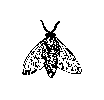
\epsfig{file=fly.eps} \caption{A sample black and white
graphic (.eps format).}
\end{figure}

\section{Conclusions}
\vspace{70 mm}
.
\vspace{10 mm}

%
% The following two commands are all you need in the
% initial runs of your .tex file to
% produce the bibliography for the citations in your paper.

\bibliographystyle{abbrv}
\bibliography{sigproc}  % sigproc.bib is the name of the Bibliography in this case
% You must have a proper ".bib" file
%  and remember to run:
% latex bibtex latex latex
% to resolve all references
%
% ACM needs 'a single self-contained file'!
%
\vspace{50 mm}
\newpage
%APPENDICES are optional

\appendix
%Appendix A
\section{Headings in Appendices}
The rules about hierarchical headings discussed above for the body
of the article are different in the appendices. In the
\textbf{appendix} environment, the command \textbf{section} is
used to indicate the start of each Appendix, with alphabetic order
designation (i.e. the first is A, the second B, etc.) and a title
(if you include one).  So, if you need hierarchical structure
\textit{within} an Appendix, start with \textbf{subsection} as the
highest level. Here is an outline of the body of this document in
Appendix-appropriate form:
\subsection{Introduction}
\subsection{The Body of the Paper}
\subsubsection{Type Changes and  Special Characters}
\subsubsection{Math Equations}
\paragraph{Inline (In-text) Equations}
\paragraph{Display Equations}
\subsubsection{Citations}
\subsubsection{Tables}
\subsubsection{Figures}
\subsubsection{Theorem-like Constructs}
\subsubsection*{A Caveat for the \TeX\ Expert}
\subsection{Conclusions}
\subsection{Acknowledgments}
\subsection{Additional Authors}
This section is inserted by \LaTeX; you do not insert it. You just
add the names and information in the
\texttt{{\char'134}additionalauthors} command at the start of the
document.
\subsection{References}
Generated by bibtex from your ~.bib file.  Run latex, then bibtex,
then latex twice (to resolve references) to create the ~.bbl file.
Insert that ~.bbl file into the .tex source file and comment out
the command \texttt{{\char'134}thebibliography}.
% This next section command marks the start of
% Appendix B, and does not continue the present hierarchy
\section{More Help for the Hardy}
The sig-alternate.cls file itself is chock-full of succinct and
helpful comments.  If you consider yourself a moderately
experienced to expert user of \LaTeX, you may find reading it
useful but please remember not to change it.
%\balancecolumns % GM June 2007
% That's all folks!

\balancecolumns
\end{document}
